\documentclass[a4paper,11pt]{article}
\usepackage[swedish]{babel} % Ändrar Table of contents till innehållsförteckning etc
\usepackage[T1]{fontenc}
\usepackage[utf8]{inputenc}

\usepackage{graphicx} %Behövs för att importera bilder
\usepackage{float} %Gör så att man kan använda ´H´ attributet för bilder(funkar bättre än h!) så att bilden hamnar där man säger åt den att vara
\usepackage[space]{grffile} % Fixar så att man kan använda space i filvägar utan någon escape characters
\usepackage{nopageno} % Tar bort defalt sidnummret i botten av sidan, behövs för försättsbladet eftersom den har plain som pagestyle och inte den som jag definerat nedan
\usepackage{lastpage} % Lägger till en referens för att få fram den sista sidnummret i dokumentet
\usepackage[hidelinks]{hyperref} %Lägger till hyperlänkar vid alla refrenser och vid innehållsförtäckningen


% Hela blocket nedan är paket som behövs för att importera lister med kod
\usepackage{color}
\usepackage{xcolor}
\usepackage{listings}
\definecolor{dkgreen}{rgb}{0,0.6,0}
\definecolor{gray}{rgb}{0.5,0.5,0.5}
\definecolor{mauve}{rgb}{0.58,0,0.82}
\lstset{ %
  language=Java,                  % the language of the code
  basicstyle=\footnotesize,       % the size of the fonts that are used for the code
  numbers=left,                   % where to put the line-numbers
  numberstyle=\tiny\color{gray},  % the style that is used for the line-numbers
  stepnumber=1,                   % the step between two line-numbers. If it's 1, each line 
                                  % will be numbered
  numbersep=5pt,                  % how far the line-numbers are from the code
  backgroundcolor=\color{white},  % choose the background color. You must add \usepackage{color}
  showspaces=false,               % show spaces adding particular underscores
  showstringspaces=false,         % underline spaces within strings
  showtabs=false,                 % show tabs within strings adding particular underscores
  frame=single,                   % adds a frame around the code
  rulecolor=\color{black},        % if not set, the frame-color may be changed on line-breaks within not-black text (e.g. commens (green here))
  tabsize=4,                      % sets default tabsize to 2 spaces
  captionpos=b,                   % sets the caption-position to bottom
  breaklines=true,                % sets automatic line breaking
  breakatwhitespace=false,        % sets if automatic breaks should only happen at whitespace
  title=\lstname,                 % show the filename of files included with \lstinputlisting;
                                  % also try caption instead of title
  keywordstyle=\color{blue},          % keyword style
  commentstyle=\color{dkgreen},       % comment style
  stringstyle=\color{mauve},         % string literal style
  escapeinside={\%*}{*)},            % if you want to add a comment within your code
  morekeywords={*,...}               % if you want to add more keywords to the set
}
\lstset{
  literate={ö}{{\"o}}1
           {ä}{{\"a}}1
           {å}{{\aa}}1
}%Översätter inputlistings output till utf8


\usepackage{fancyhdr} % Användsa för att göra egna sidhuvuden/sidfötter
\fancyhf{} %  Tömmer standardinnehållet i header footer
\setlength{\headheight}{27mm} % Om du använder en bild så se till att den får plats i sidhuvudet. Latex skapar altid mer plats till text däremot.
\fancyhead[L]{\includegraphics[height=25mm]{C:/Users/Ralle/Documents/ChatProjectReport/MAH.png}}
\fancyhead[R]{Objektorienterad programutveckling,\\ trådar och datakommunikation \\Projekt Chatapplikation}

\fancyfoot[L]{\today}
\fancyfoot[R]{Sida \thepage\ av \pageref{LastPage}}

\title{Projektrapport\\
\large{Chattapplikation}\\
\large{för Objektorienterad programutveckling, trådar och datakommunikation} }
\author{Rasmus Andersson\\Emil Sandgren\\Erik Sandgren\\Jimmy Maksymiw\\Lorenz Puskas\\Kalle Bornemark}
\makeindex
\begin{document}

\pagestyle{fancy}
\maketitle
\newpage
\tableofcontents
\newpage

\section{Arbetsbeskrivning}

\subsection{Rasmus Andersson} 
Arbetade med kommunikation mellan servern och klienten med Kalle Bornemark, och Jimmy Maksymiw. Formgav projektrapporten samt skrev ImageScaleHandler.java samt Chatlog.java. Jobbade inte med UI-klasserna.

\subsection{Emil Sandgren} 
% Skriv här
\subsection{Erik Sandgren} 

Arbetat med generell grundläggande kommunikation mellan server och klient i början. Jobbat sedan med UI och hoppat in lite därefter på det som behövdes. Har ritat upp strukturen mycket och buggfixat.

\subsection{Jimmy Maksymiw} 
Arbetat med planering och struktur av hur chatten ska fungera. Med programmeringen har jag arbetat mest med logiken som används i både klienten och servern. Hur kommunikationen sker och vad som ska göras på de olika sidorna. Har också varit med och gjort de olika diagrammen. 
\subsection{Lorenz Puskas} 
Arbetade enbart med att designa ClientUI tillsammans med Emil.
\subsection{Kalle Bornemark} 
Arbetat med server/klient-kommunikation, projektplanering och klasstrukturen. Skapade även diagrammen och fungerat som projektledare till och från.

\section{Instruktioner för programstart}
För att köra programmet så krävs det att man startar en server och minst en klient. Main-metoden för att starta servern finns i StartServer.java och main-metoden för att starta klienter finns i StartClient.java. Alla filvägar är relativa till det workspace som används och behöver inte ändras.

\section{Systembeskrivning}

Vårt system förser en Chatt-tjänst. I systemet finns det klienter och en server. Klienterna har ett grafiskt användargränssnitt som han eller hon kan använda för att skicka meddelanden till alla andra anslutna klienter, enskilda klienter, eller till en grupp av klienter. Meddelanden består av text eller av bilder. Alla dessa meddelanden går via en server som ser till att meddelanden kommer fram till rätt gruppchat eller till lobbyn. Servern lagrar alla textmeddelande som användarna skickar och loggar även namnet på de bilder som skickas via bildmeddelanden. Det loggas även när användare ansluter eller stänger ner anslutningen mot servern.

\section{Klassdiagram}
\subsection{Server}
	\begin{figure}[H]
		\centering
		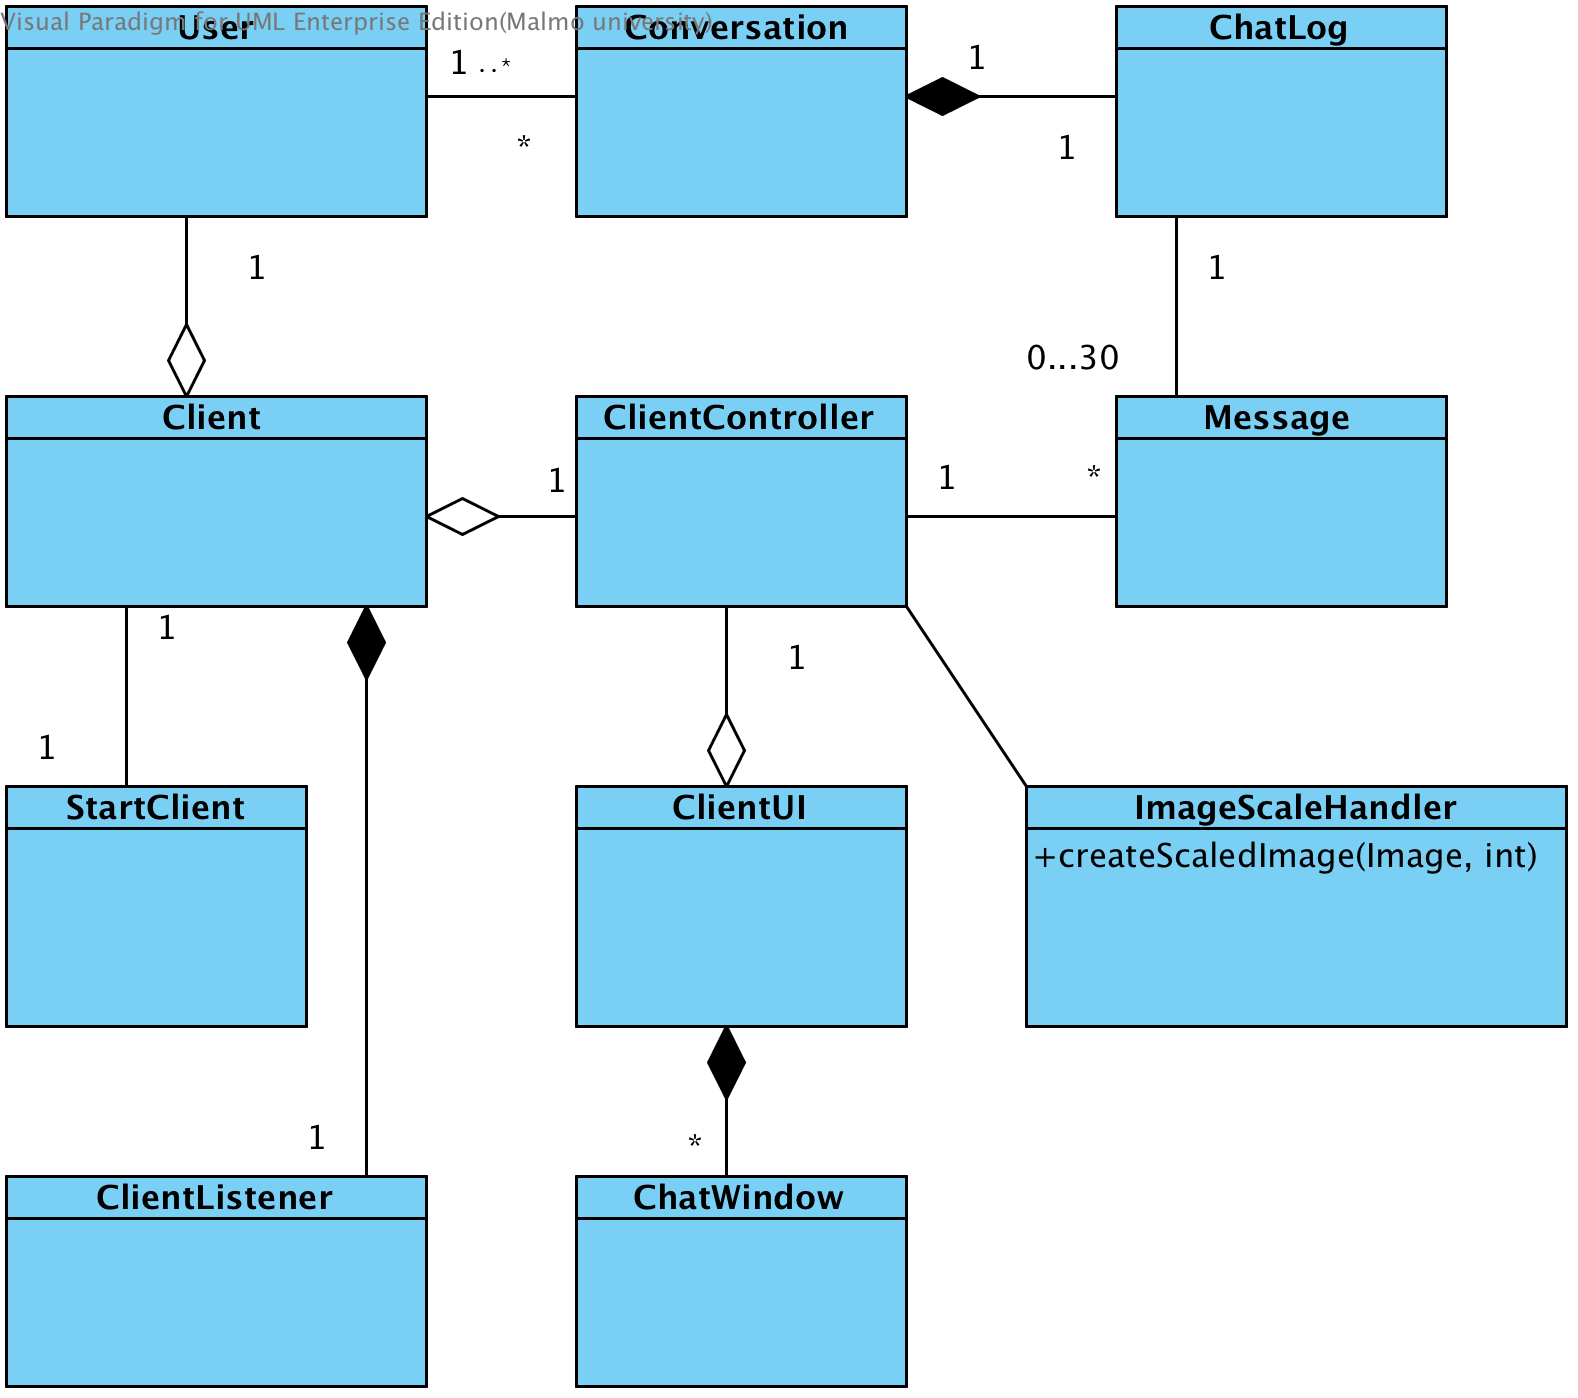
\includegraphics[width=\textwidth]{diagram/Client.png}
		\caption{Server}

	\end{figure}
\subsection{Klient}
	\begin{figure}[H]
		\centering
		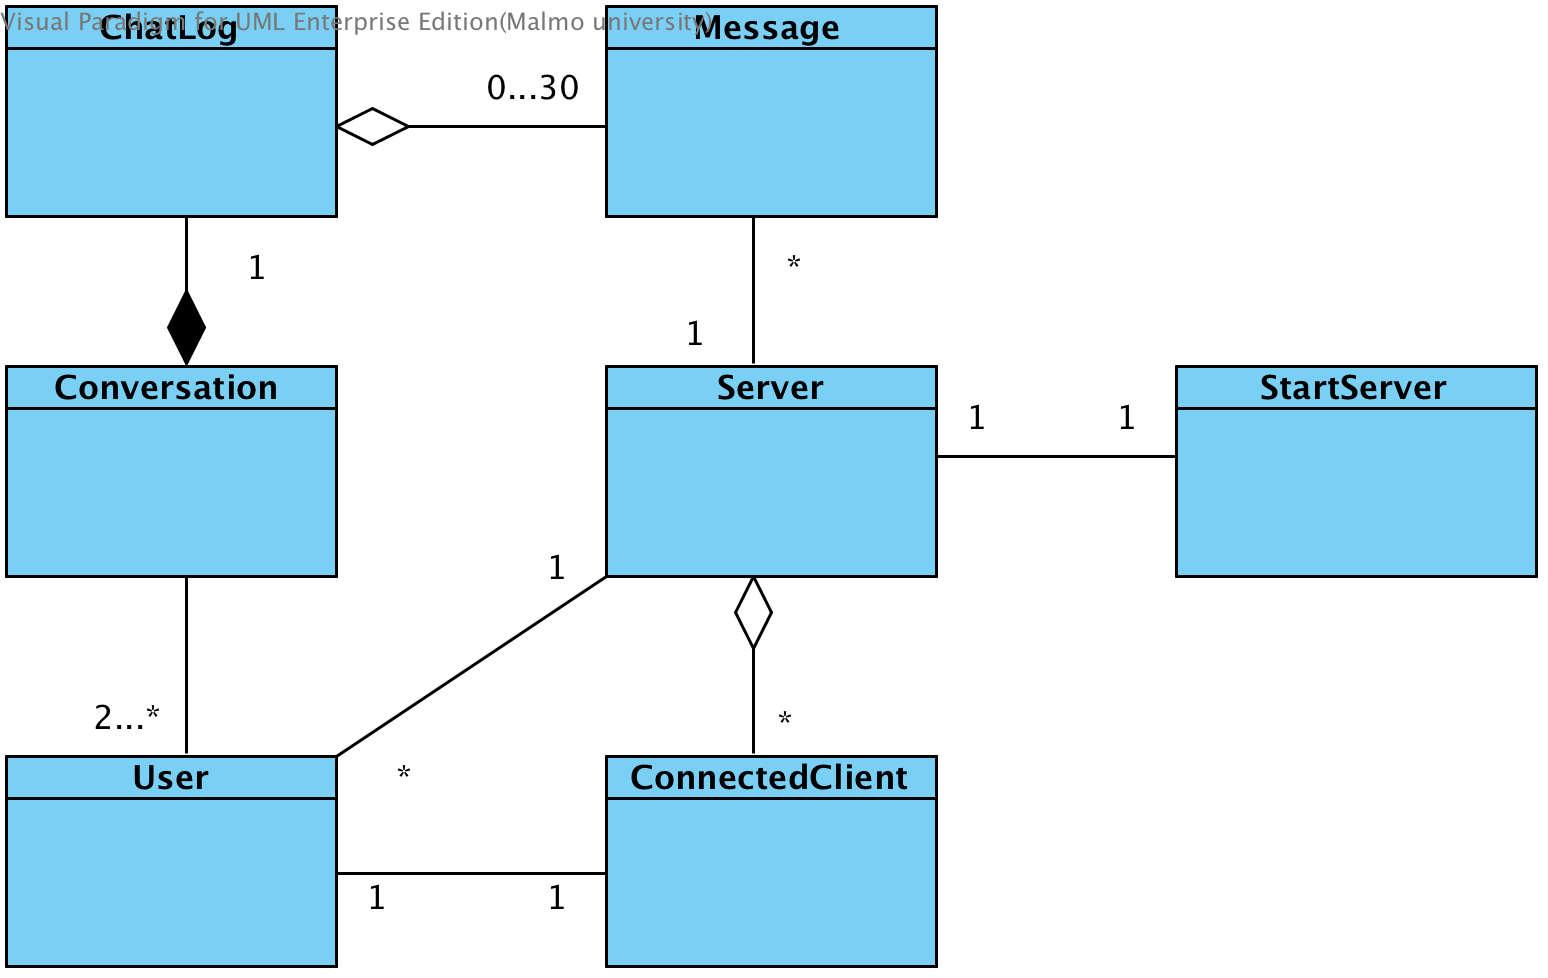
\includegraphics[width=\textwidth]{diagram/Server.png}
		\caption{Klient}
	\end{figure}
\section{Kommunikationsdiagram}

	\subsection{Connect and login}
	\begin{figure}[H]
		\centering
		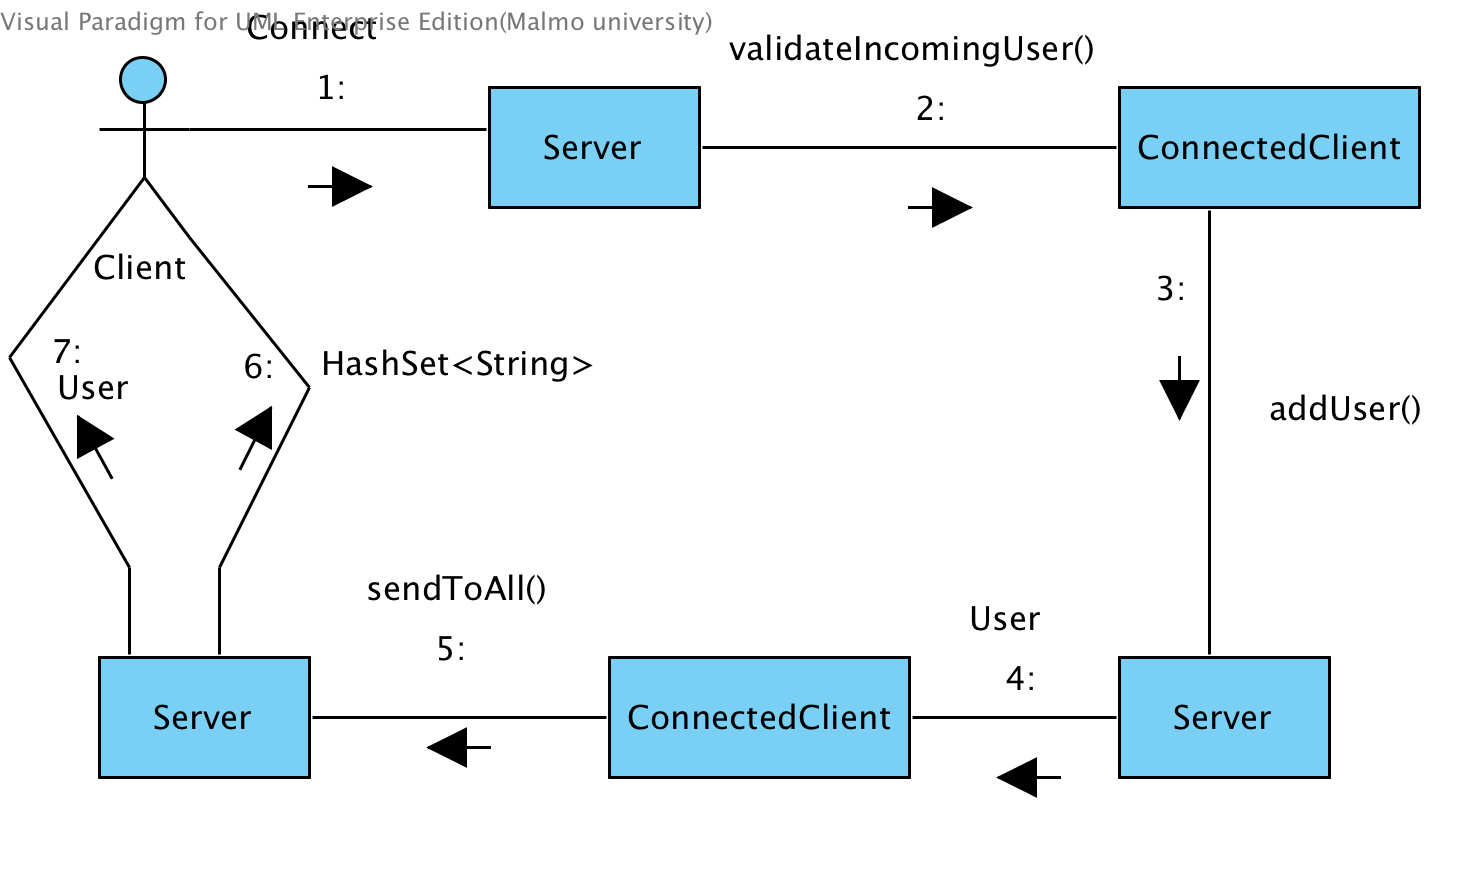
\includegraphics[width=\textwidth]{diagram/Server_ConnectAndLogin2.png}
		\caption{Client connecting and logging in}
	\end{figure}


	\subsection{Client send Message}
	\begin{figure}[H]
		\centering
		\includegraphics[width=\textwidth]{diagram/Client_sendMessage2.png}
		\caption{Client sending a message}
	\end{figure}
\section{Sekvensdiagram}
\subsection{Connect and login}
	\begin{figure}[H]
		\centering
		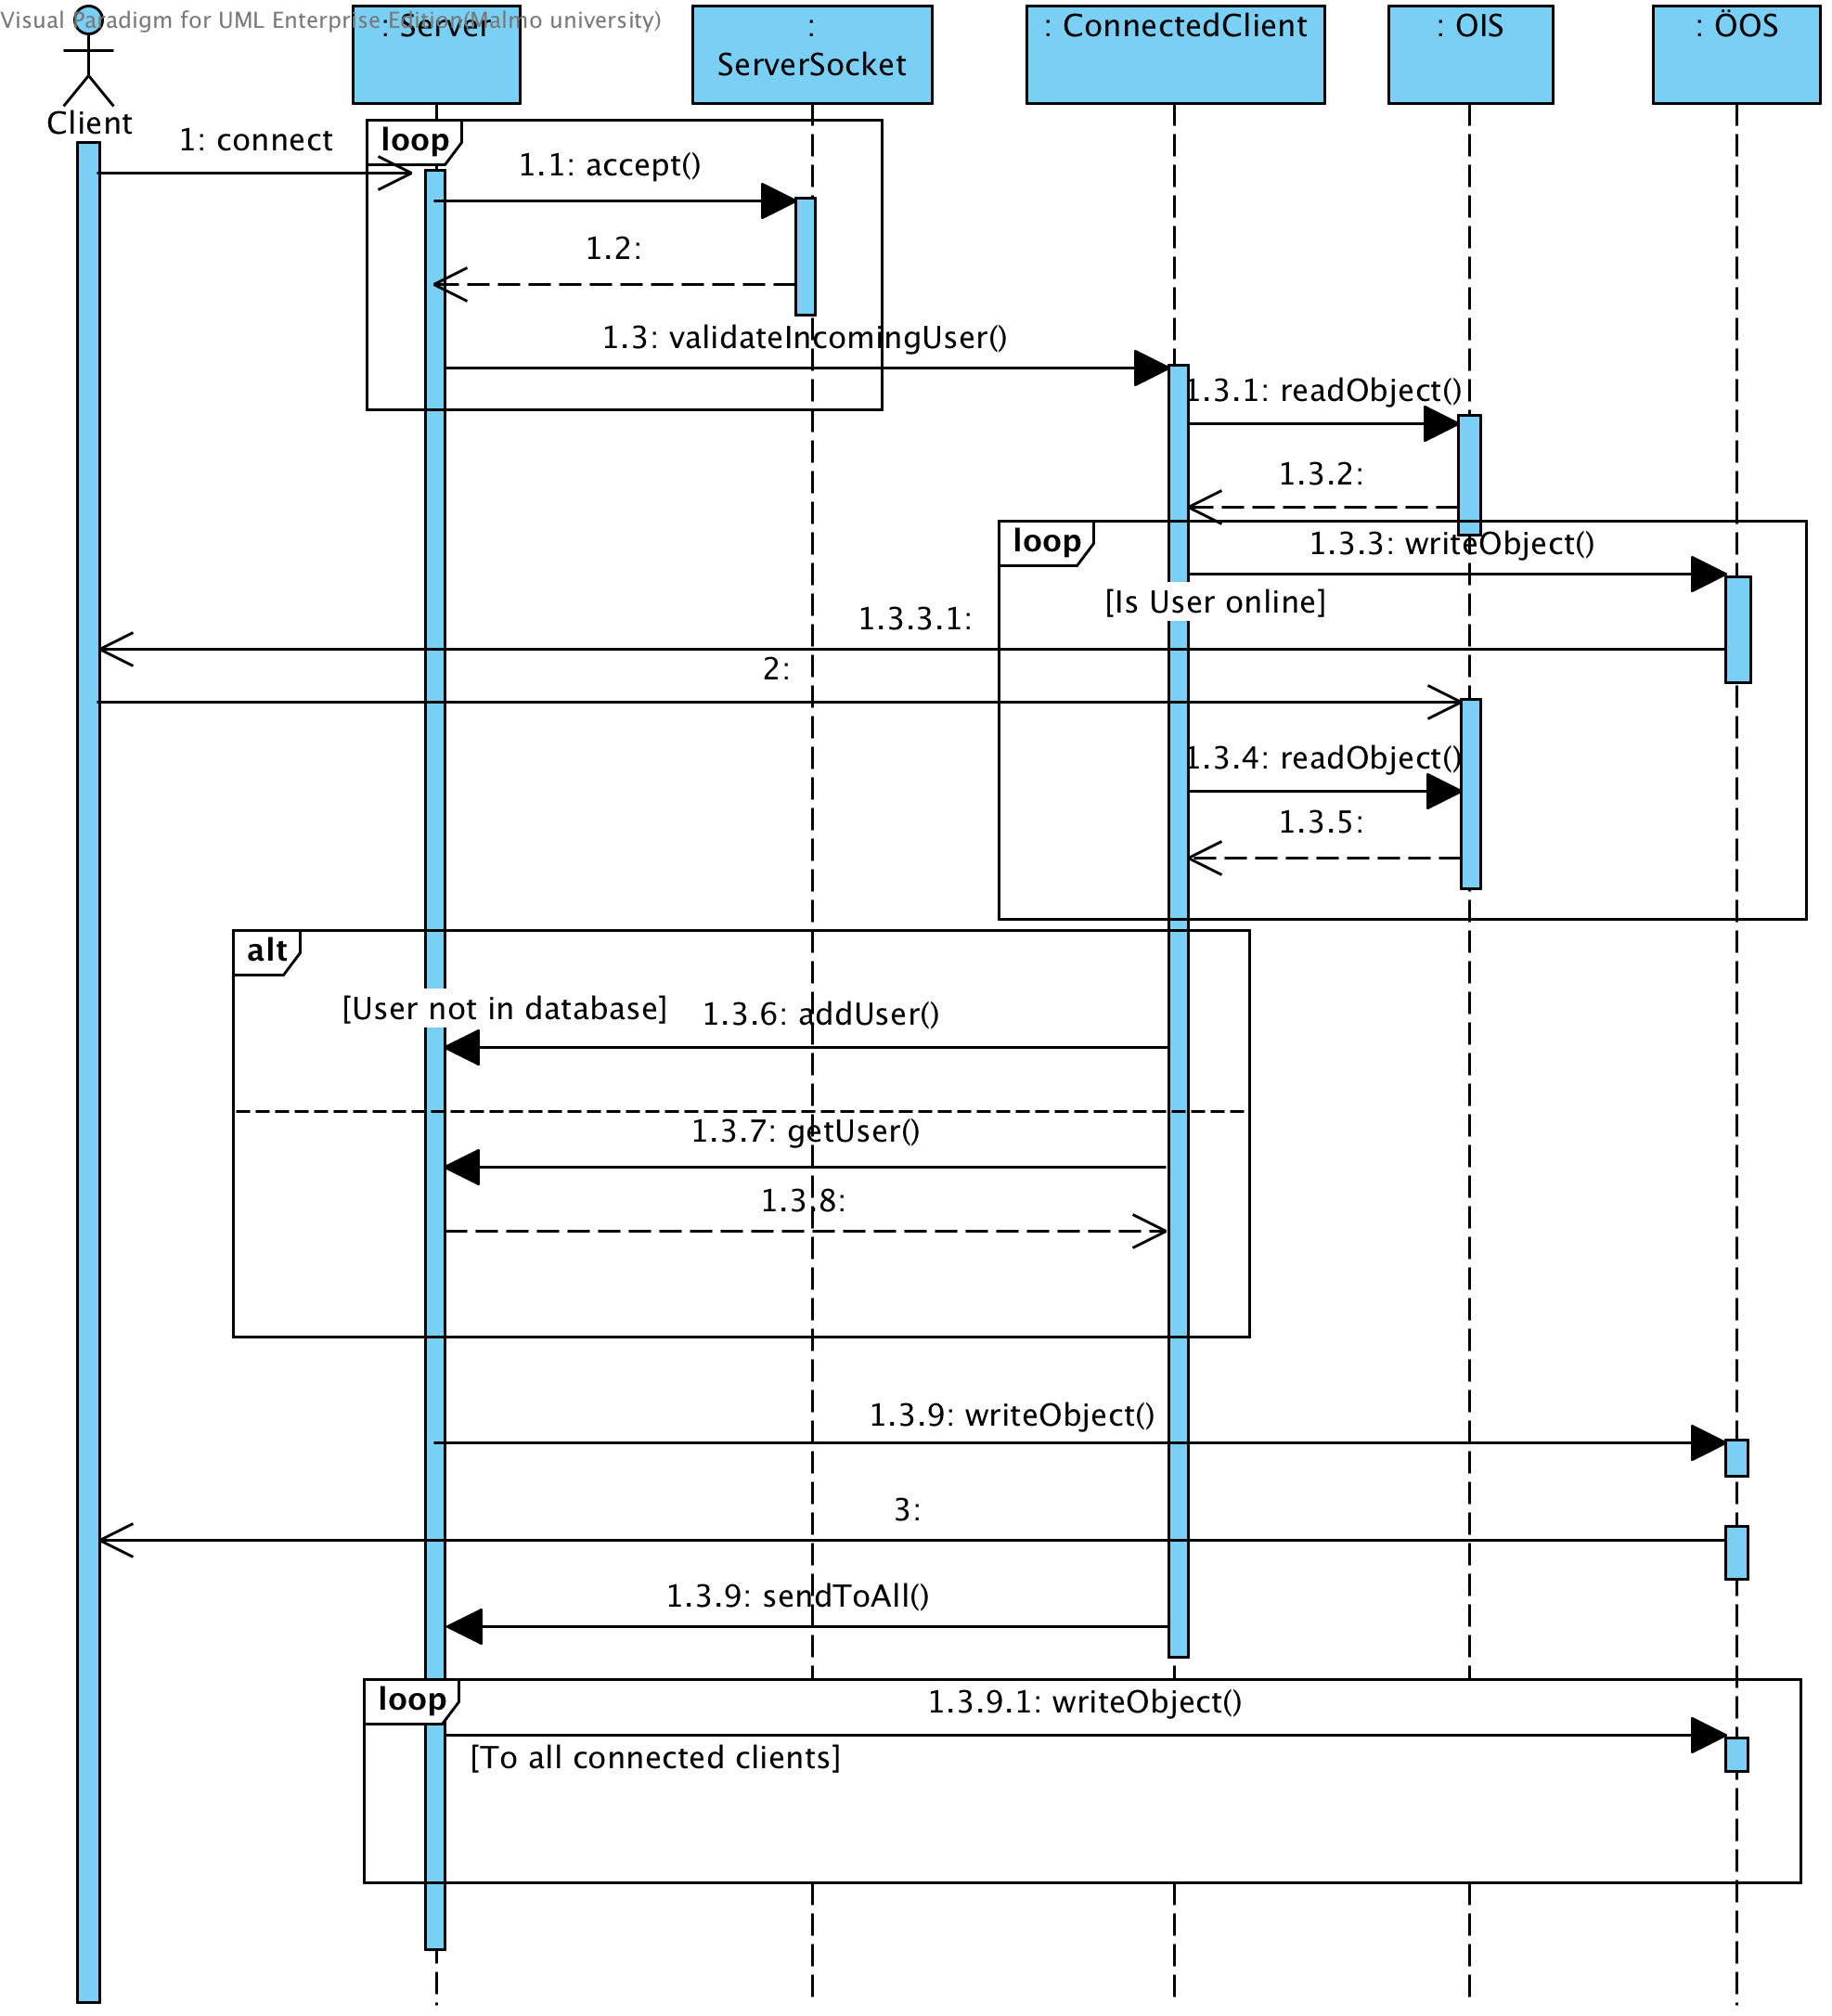
\includegraphics[width=\textwidth]{diagram/Server_ConnectAndLogin.png}
		\caption{Client connecting and logging in}
	\end{figure}


\subsection{Send message}
	\begin{figure}[H]
		\centering
		\includegraphics[width=\textwidth]{diagram/Client_sendMessage.png}
		\caption{Client sending a message}
	\end{figure}


\section{Källkod}

	\subsection{Server}
		\subsubsection{Server.java, Server.ConnectedClient.java}
		\lstinputlisting[language=java,caption=Server]{../../chat/Server.java}
		\subsubsection{Startserver.java}
		\lstinputlisting[language=java,caption=StartServer]{../../chat/Startserver.java}
		
	\subsection{Klient}
		\subsubsection{ChatWindow.java}
		\lstinputlisting[language=java,caption=ChatWindow]{../../chat/ChatWindow.java}
		\subsubsection{Client.java}
		\lstinputlisting[language=java,caption=Client]{../../chat/Client.java}
		\subsubsection{ClientController.java}
		\lstinputlisting[language=java,caption=ClientController]{../../chat/ClientController.java}
		\subsubsection{ClientUI.java}
		\lstinputlisting[language=java,caption=ClientUI]{../../chat/ClientUI.java}
		\subsubsection{ImageScaleHandler.java}
		\lstinputlisting[language=java,caption=ImageScaleHandler]{../../chat/ImageScaleHandler.java}
		\subsubsection{StartClient.java}
		\lstinputlisting[language=java,caption=LoginUI]{../../chat/StartClient.java}

	\subsection{Delade klasser}
		\subsubsection{ChatLog}
			\lstinputlisting[language=java,caption=ChatLog]{../../chat/ChatLog.java}
			\subsubsection{Message}
			\lstinputlisting[language=java,caption=Message]{../../chat/Message.java}
			\subsubsection{User}
			\lstinputlisting[language=java,caption=User]{../../chat/User.java}
			\subsubsection{Conversation}
			\lstinputlisting[language=java,caption=Conversation]{../..//chat/Conversation.java}








	
\end{document}
